\documentclass[12pt,letterpaper]{article}
\usepackage[utf8]{inputenc}
\usepackage[spanish]{babel}
\usepackage{amsmath}
\usepackage{amsfonts}
\usepackage{amssymb}
\usepackage{makeidx}
\usepackage{graphicx}
\usepackage[left=2cm,right=2cm,top=2cm,bottom=2cm]{geometry}
\author{john negrete}
\title {primer avance}

\begin{document} 

\title {primer avance}

\section*{                  ...(PRIMER AVANCE)... }
\section*{John Negrete..........(7-B)}
\section*{Benjamin Enciso..........(ing.Mecatronica)}
\section*{Leonardo Contreras.......(cinematica de robots)}
\section*{Martin Barajas......(Moran Garabito)}

\includegraphics[scale=1]{upz.jpg}
\newpage 
\section*{planteamiento}

Se decidió hacer este proyecto (brazo soldador) porque se ha detectado sobre la imprecisión y la impureza de los operarios al momento de soldar alguna pieza con soldadura MMA, recabando información se contempla que de igual manera hay un gran número de accidentes provocadas en este oficio de soldador.
\\\\
Los soldadores son miembros de un grupo ocupacional que está expuesto a diferentes tipos de riesgos, como gases y polvos en la soldadura. 
\\\\
En algunas condiciones, es por los gases emitidos por algunos electrodos, así como los vapores que emanan algunos metales durante la soldadura, estos pueden causar daño por inhalación en los soldadores, desde una simple irritación nasal, hasta un problema permanente en el sistema respiratorio.
\\\\
El choque eléctrico es uno de los principales peligros a que se expone un soldador, ya que, al hacer contacto con una corriente eléctrica, recibe una descarga que le puede ocasionar una reacción violenta, en algunas ocasiones puede ser inofensiva y en otras mortal.
\\
El dejar el equipo energizado cuando no se está utilizando, no utilizar guantes al manejar el equipo o pararse sobre agua cuando se está soldando, son las principales razones por la que se pude llevar a cabo una descarga o choque eléctrico.
\\\\
Lo que se planea con el robot es tener la posibilidad de mejorar los puntos de soldadura, hacerlos más precisos, más exactos, más limpios y sobre todo manejar el microalambre desde una distancia más segura.

\newpage




\section*{introduccion}
Un robot puede ser definido como una máquina que efectúa un número de trabajos, mediante la programación previa. Una peculiaridad de los robots es su estructura de un brazo mecánico y otra su adaptabilidad a diferentes herramientas.
\\\\
Por siglos el ser humano ha construido máquinas que imiten las partes del cuerpo humano. Los antiguos egipcios unieron brazos mecánicos a las estatuas de sus dioses.
\\\\ 
Estos brazos fueron operados por sacerdotes, quienes clamaban que el movimiento de estos era inspiración de sus dioses. Los griegos construyeron estatuas que operaban con sistemas hidráulicos, los cuales se utilizaban para fascinar a los adoradores de los templos.
\\\\
El uso de sistemas robóticos en la industria, para cumplir funciones que requieren extrema precisión ha ido en ascenso en las últimas décadas como también en el uso personal y familiar.
\\\\
El desarrollo de estos sistemas se ha enfocado en mejorar ciertos aspectos como resistencia para trabajar en diferentes condiciones, precisión con la que se realizan movimientos, multifuncionalidad (manipulación, corte, perforación, etc.), adaptabilidad en diferentes entornos de trabajo.
\\\\
Por lo tanto, dados todas estas utilidades, el diseño propio y construcción de prototipos de brazo robótico para manipulación, posicionamiento, corte láser o escaneo tengan un costo accesible tanto para la industria como para la educación, es un buen tema a considerar como proyectos de desarrollo, por estudiantes de ingeniería mecatrónica.
\\\\
El desarrollo en la tecnología, donde se incluyen las computadoras, los actuadores de control retroalimentados, transmisión de potencia a través de engranes, y la tecnología en sensores han contribuido a flexibilizar los mecanismos autómatas para desempeñar tareas dentro de la industria. La investigación en inteligencia artificial desarrolló maneras de emular el procesamiento de información humana con computadoras electrónicas.

\newpage
\subsection*{justificacion}
El hecho de soldar de manera automatizada con microalambre va a resolver problemáticas importantes para el operario, tales como la reducción de tiempo muerto entre soldar dos materiales y ensamblar piezas o esmerilarlos para quitar la escoria y dejar la soldadura limpia, esto podrá ser un proceso semiautomático o automático que sea menos dependiente de la habilidad de operador, se pretende que no solo sea una herramienta de fácil uso para el sexo masculino sino también para el femenino aumentando así la cantidad, calidad, tiempo de trabajo y de igual manera  apoyar la inclusión.
\\\\
Un factor importante en el proyecto es usar MIC/MAC ya que es intrínsecamente más productiva que la soldadura MMA en la que se hace una parada cada vez que se consume el electrodo además de hacer poca formación de gases contaminantes y tóxicos.
\\\\
Las principales bondades de este proceso son la alta productividad y excelente calidad; en otras palabras, se puede depositar grandes cantidades de metal (tres veces más que con el proceso de electrodo revestido) con una buena calidad.


\section*{meta}
Incorporar una soldadora de micro alambre en un brazo robótico


\subsection*{objetivos}
\begin{flushleft}
Diseñar las piezas
\end{flushleft}
\begin{flushleft}
Diseñar boceto 2D
\end{flushleft}
\begin{flushleft}
Calcular los elementos finitos
\end{flushleft}

\subsection*{preguntas de indagacion}

\begin{flushleft}
1. Cuánto tiempo se invierte en soldar?
\end{flushleft}
\begin{flushleft}
2.	¿Qué riesgos se pueden ocacionar a la hora de soldar?
\end{flushleft}
\begin{flushleft}
3.	¿Qué protección se utiliza?
\end{flushleft}
\begin{flushleft}
4.	¿Es dificil poner un buen cordón de soldadura?
\end{flushleft}

\newpage
\section*{resultados}

Basados en la investigacion el tiempo empleado para soldar un material va a depender de varios factores tales como el grosor del material, el voltaje en la corriente eléctrica, los centímetros o la distancia que se desea soldar, la altura en la que se pueda estar colocado y la posicion que suele complicar la labor. 
También los riesgos, el hecho de que puede ser peligroso si no se utiliza la protección adecuada y aun cuando se usa no es garantía de que pueda pasar alguna lesión.
\\\\
La proteccion que se utiliza es: máscara para soldar, cubre bocas o paliacate y guantes de cuero al soldar horizontal y verticalmente, no obstante, al soldar boca arriba se necesita una camisola y una capucha para disminuir el riesgo de las quemaduras.
\\\\
Es un trabajo que puede realizar cualquier persona más sin embargo el aprender este oficio lleva tiempo ya que más que nada se hace a prueba y error lo que en ocasiones genera pérdidas de material y tiempo que no genera ganancias.
\\\\
Según estudios del departamento de empleo y asuntos sociales del gobierno Vasco, seguridad y salud laborales los humos de soldadura son una mezcla de partículas y gases generados por el fuerte calentamiento de las sustancias presentes en el entorno del punto de soldadura.
\\\\
Estas sustancias son fundamentalmente:
\\\\
-Las piezas a soldar 
\\
-los posibles recubrimientos 
\\
-Los materiales de aporte utilizados en el proceso de soldadura 
\\
-El aire en la zona de soldadura y su posible contaminación

\begin{center}
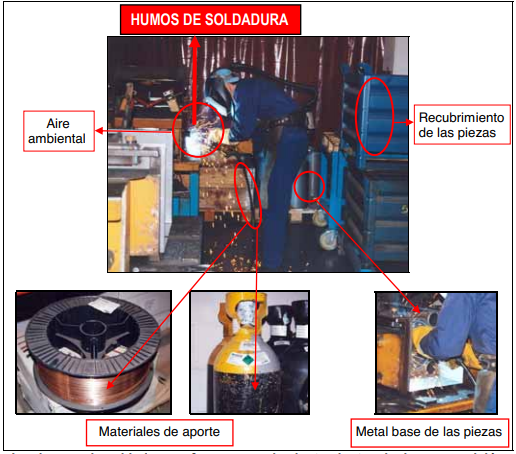
\includegraphics[scale=0.7]{imag1.png} 
\end{center} 
\begin{center}
Figura 1. Ejemplo de factores contaminantes.
\end{center}



\newpage
En la postura que adopta el soldador durante su trabajo hay dos aspectos de gran repercusión en la cantidad de humos inhalados:
\\\\
- Su posición con respecto a la vertical del punto de soldadura. 
\\
- La distancia al punto de soldadura.
\\\\
Cuando el soldador adopta una postura tal que su cara queda justo en la vertical del punto de operación, los humos inciden directamente sobre él y la cantidad de ellos que inhala es muy superior a cuando mantiene su cara apartada de la corriente ascendente de humos.
\\\\
La inhalación de humos de soldadura puede ocasionar daños para la salud. Los órganos afectados y la gravedad de las lesiones dependen de los contaminantes presentes en los humos y de la cantidad inhalada. 
Cada contaminante tiene asignada una concentración máxima en el aire, conocida como Valor Límite Ambiental (VLA), (Ver gráfico 1) por debajo del cual se considera que, en base a los conocimientos actuales sobre su toxicidad, la mayoría de los trabajadores expuestos durante toda su vida laboral, no sufrirán trastornos en su salud.
\\\\
En la medida que se superen estos límites aumentarán las probabilidades de que los daños se manifiesten. Para algunos de los contaminantes que pueden estar presentes en los humos de soldadura, tales como el cromo, el cadmio, los fluoruros y el monóxido de carbono, se dispone también de Valores Límites Biológicos (VLB), por lo que, mediante análisis de sangre, orina o aire exhalado, pueden obtenerse datos de la exposición complementarios a los muestreos ambientales. 
\\\\
En la tabla 1 se indican los principales efectos perjudiciales derivados de la inhalación de los humos de soldadura, que para ofrecer una visión general los clasificaremos en:
\\
Efectos agudos, crónicos, sensibilizantes, cancerígenos y teratógenos.

\begin{center}
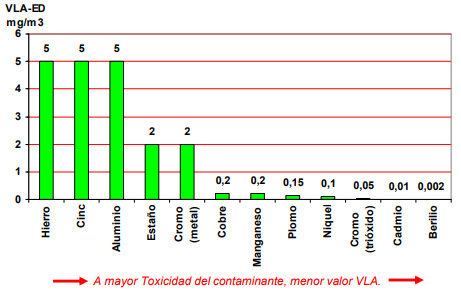
\includegraphics[scale=1]{imag2.png}  
\end{center}
\begin{center}
Grafica 1. Límites de exposición profesional de algunos humos metálicos de soldadura. (Año 2009)
\end{center}

\newpage
\begin{flushleft}
Puestos de trabajo más accidentados: 
La gráfica muestra que los jornales y los carpinteros de obra gruesa, son los puestos de trabajo que con mayor frecuencia se accidentan, seguido por los enfierradores y los señaleros o rigger
\end{flushleft}
\begin{center}
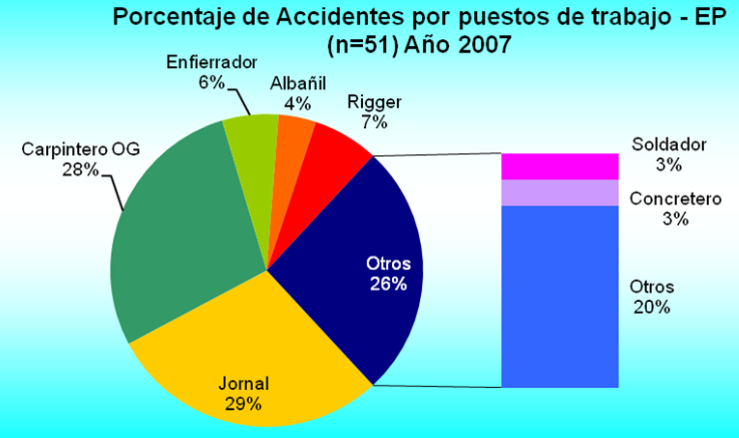
\includegraphics[scale=0.9]{imag3.png}  
\end{center}
\begin{center}
Grafica 2. Porcentaje de accidentes por puestos de trabajo.
\end{center}

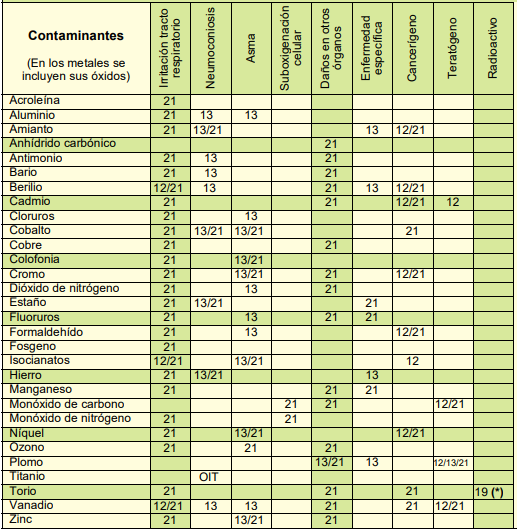
\includegraphics[scale=1.3]{imag4.png}  

\begin{center}
Tabla 1. Efectos patológicos característicos de algunos contaminantes frecuentes en los humos de la soldadura. (Orientativa)
\end{center}

\newpage

Desarrollo.
\\\\

Para el brazo se presenta una articulación con movimiento rotacional y dos angulares. Aunque el brazo articulado pueda realizar el movimiento llamado interpolación lineal (para lo cual requiere mover simultáneamente dos o tres de sus articulaciones), el movimiento natural es el de interpolación por articulación, tanto de rotacional como angular.
\\
Se denomina cinemática directa a una técnica que es utilizada en gráficos 3D por computadora, para solucionar y calcular la posicion de partes de una estructura articulada a partir de sus elementos fijos y las transformaciones que se provocan por las articulaciones de la estructura.
\\\\
La cinemática inversa se refiere a la utilización de las ecuaciones cinemáticas de un robot
para determinar los parámetros comunes que proporcionan una posicion deseada del efector
final.
\\
Especificación del movimiento de un robot de manera que su extremo efector logra una
tarea deseada es conocido como planificación de movimientos. La cinemática inversa transforma el plan de movimiento en trayectorias del actuador en conjuntos para el robot.
\\\\
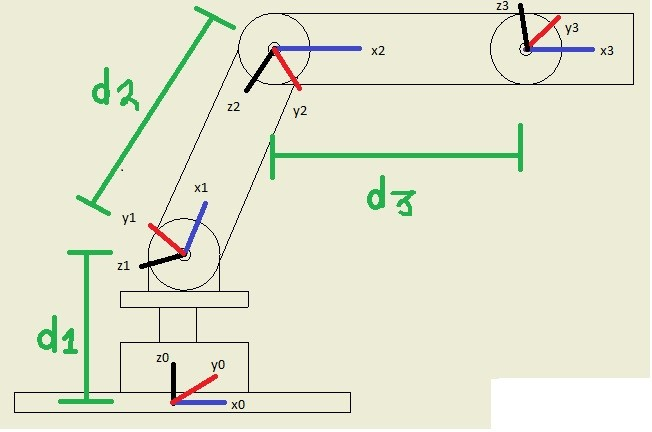
\includegraphics[scale=1]{imag6.jpg} 
\begin{center}
Figura 1.Angulos del robot
\end{center}
Se realizó el boceto 2D el cual se realizó para sacar los ángulos y la distancia del robot como se muestra en la figura 1.
Robot antropomórfico con tres grados de libertad. El robot se moverá en X y Y, así realizando los movimientos que se le indique ya que este se le colocará las pinzas de la soldadura por encima del robot en el ultimo eslabon.
\\
En la parte de la tabla 3, el apartado de los (I) es el número de los eslabones que tiene el robot. La (di y i) es la distancia que tiene cada ángulo entre sí. El (0) es la rotación de los codos y articulaciones.
Con esto obtenido se sacaron los ángulos de rotación mostrados en la tabla 1.

\begin{center}
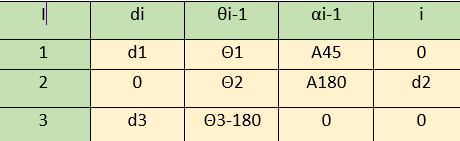
\includegraphics[scale=1]{imag7.PNG}
\end{center}

Se instaló el software inventor para realizar las piezas del robot. Lo primero que se realizo fue la base figura 1.1, fue complicado el realizamiento de la misma por la forma que tiene ya que dentro se tuvo que hacer un acoplamiento para colocar el motor principal, cuenta con tres apartados para que se le coloquen los tornillos y así pueda quedar ensamblado en una superficie plana para evitar todo tipo de movimiento.
\\\\
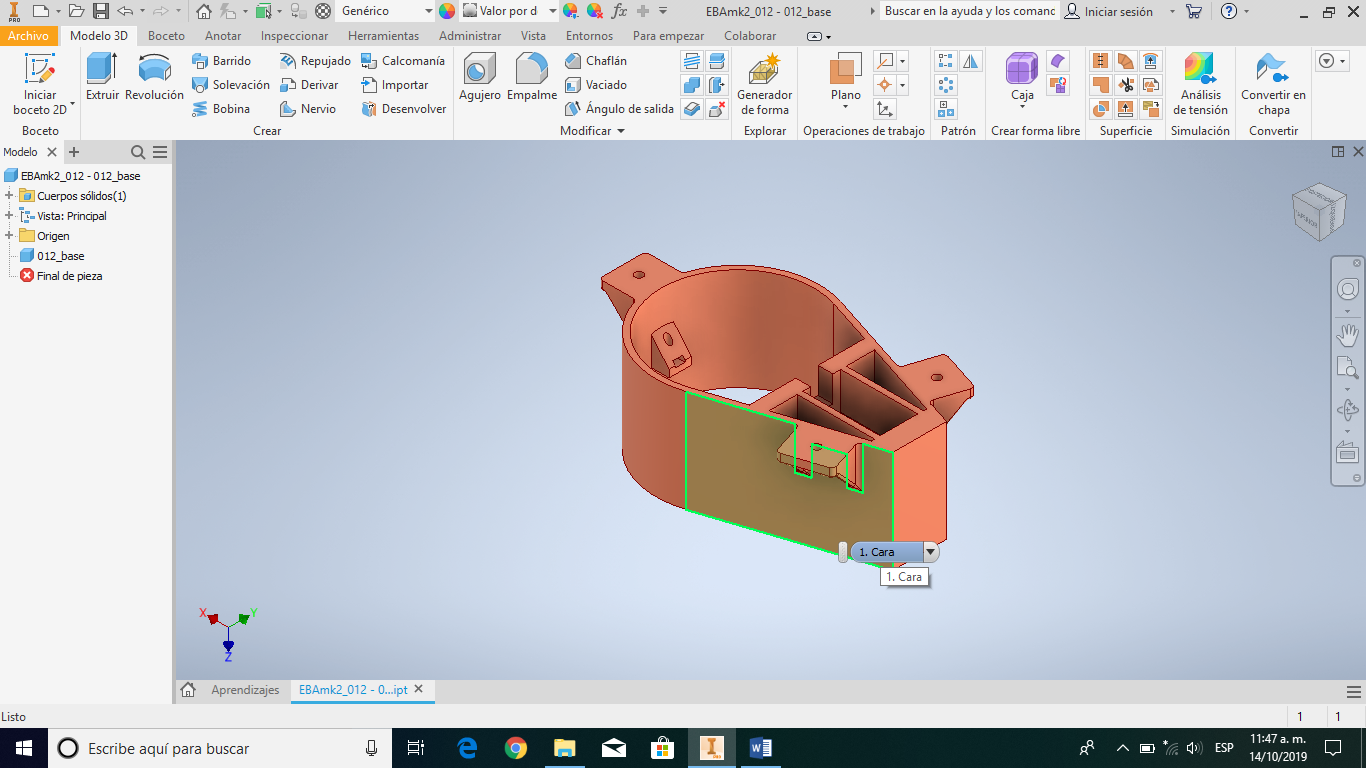
\includegraphics[scale=0.5]{imag8.png} 
\begin{center}
Figura 1.1 Base del robot.
\end{center}
La figura 1.2 consiste en una pieza que va situada sobre la base y se conectara con el motor para que despues pueda realizar una rotacion del primer eslabon.
\newpage
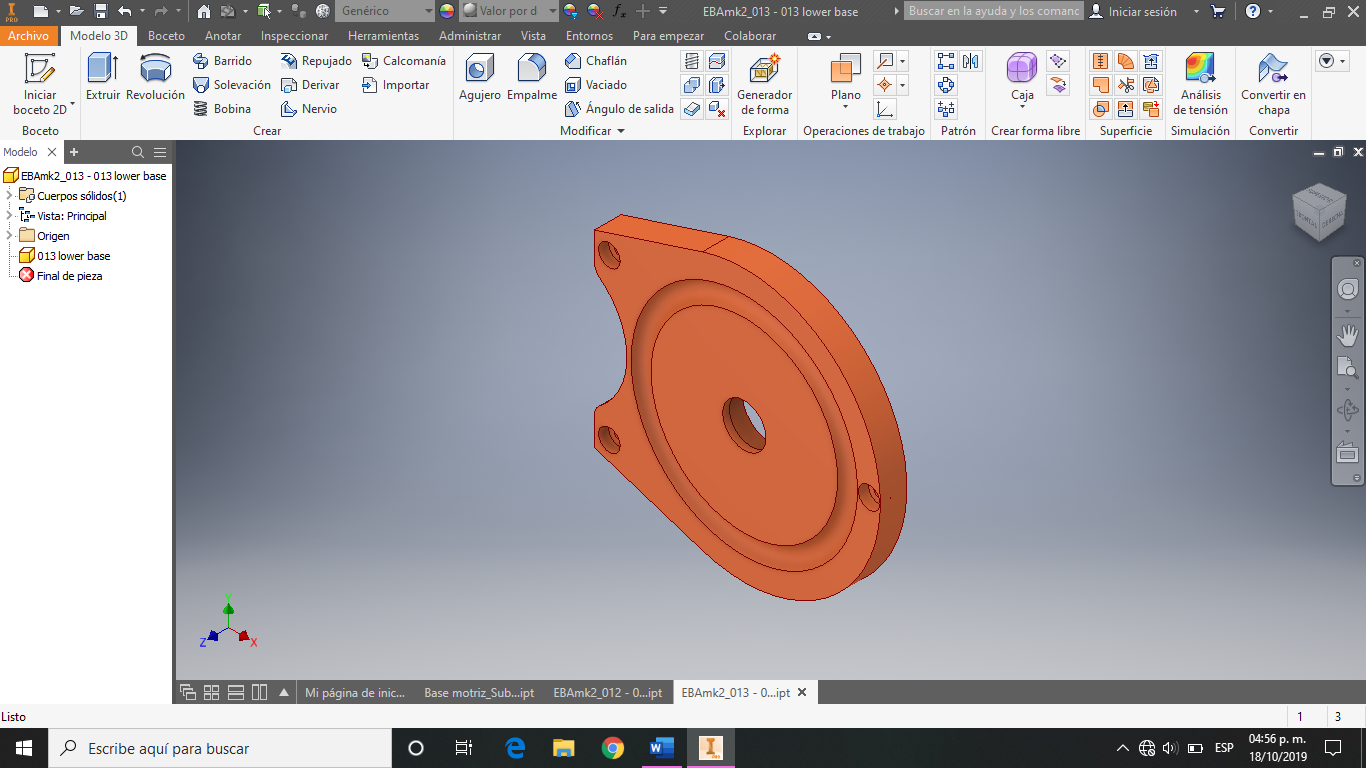
\includegraphics[scale=0.47]{image9.png}  
\\
\begin{center}
Figura 1.2 Tapadera de la base.
\end{center}
Tambien se realizo la simulacion del serv motor figura 1.3, para tener una idea mas precisa del ensamblado final dentro de la base y tambien colocarlo en otras partes del robot ya que este motor se utilizo para diseñar el acoplamiento de los demas grados de livertad.
\\\\
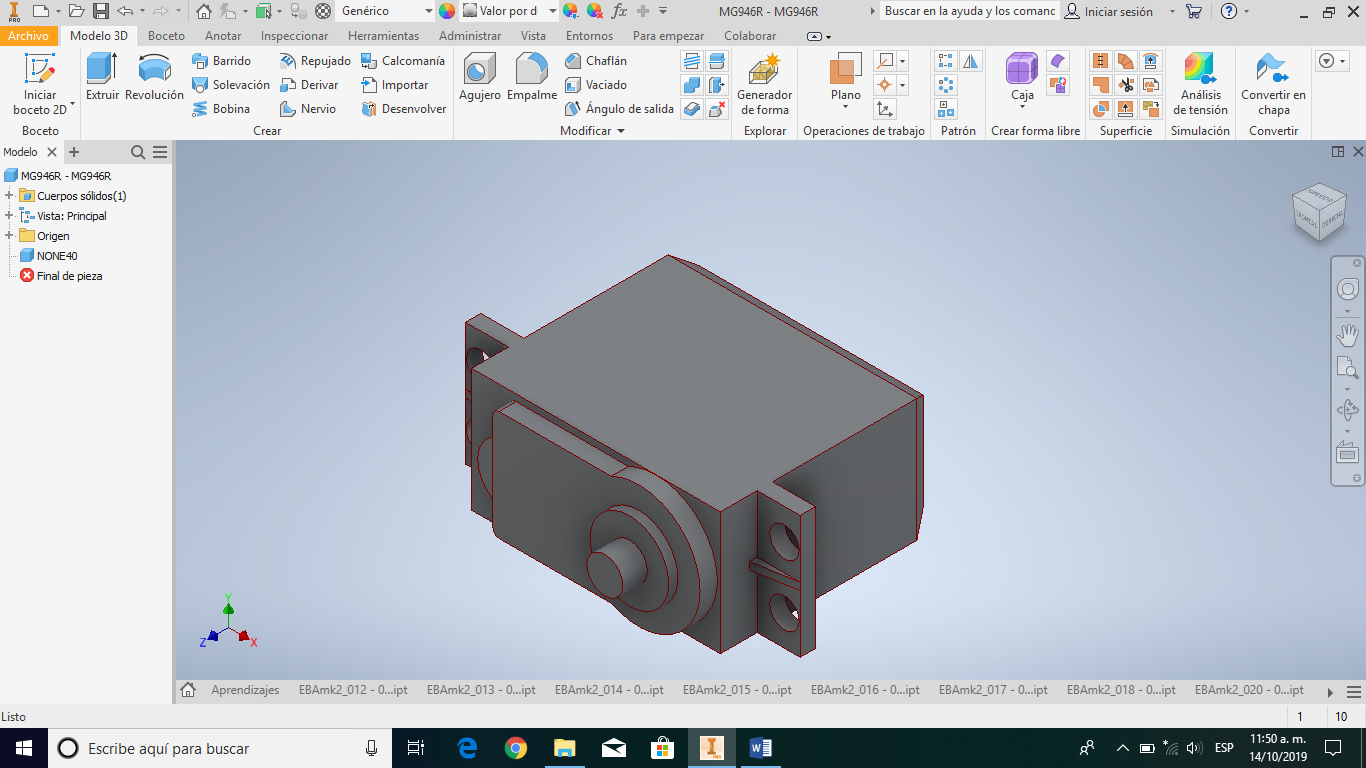
\includegraphics[scale=0.47]{imag10.png} 
\begin{center}
Figura 1.3 Servo Motor.
\end{center}

\newpage
Una vez teneiendo la base hecha la siguiente figura que se realizo fue la la base rotatoria figura 1.4, la cual se coloco arriba de la base, esta permite que se mueva todo el brazo en sentido rotacional y posteriormente se eleven los primeros dos eslabones en sentido vertical.
\\\\
\begin{center}
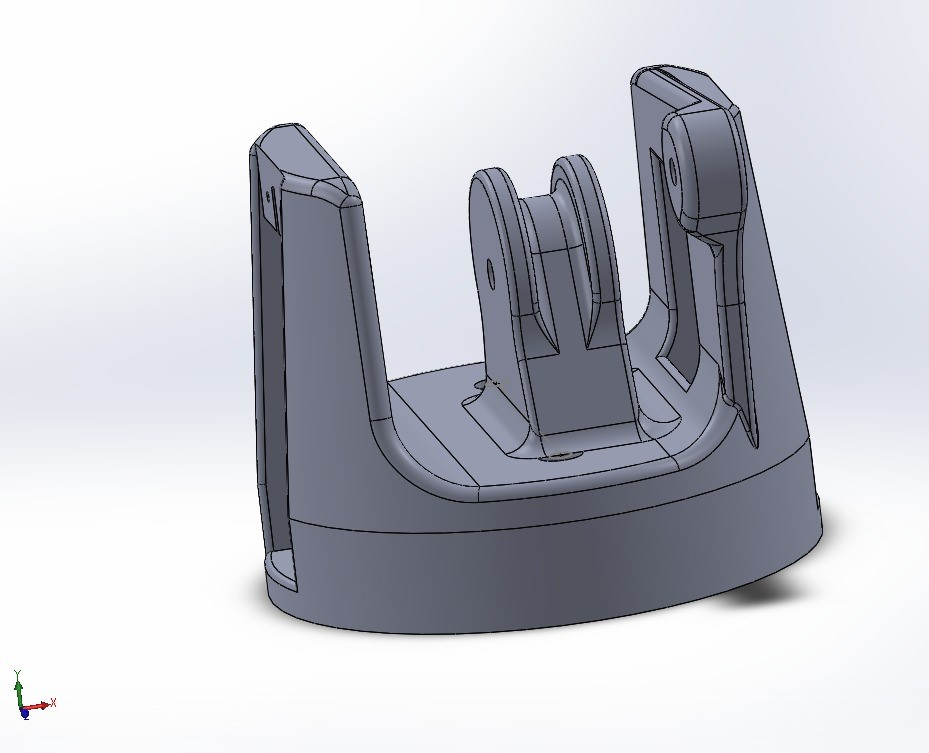
\includegraphics[scale=0.5]{img11.jpg} 
\end{center}
\begin{center}
Figura 1.4 Base rotatoria del primer eslabon.
\end{center}


\newpage
Matriz de posibles materiales y costos
\\\\
Matriz de roles
\\\\
Diagrama GANTT de tiempos y actividades
\\\\
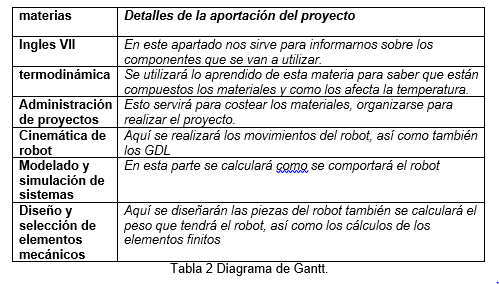
\includegraphics[scale=1.3]{imag5.PNG}  
\\\\
Conclusiones
\\\\
Martin Barajas.
\\\\
Realizar la parte de las piezas fue poco tedioso ya que algunas son complicadas a la hora de realizarlas. El programa que se utilizo para las piezas fue inventor, se comenzo por hacer la base la cual me llevo un tiempo porque la figura tiene muchos vertices pero con algo de ayuda  e investigacion se logro realizar esta pieza tambien a la hora de hacer los ensambles nos fue dificil porque algunas piezas no quedaban en su posocion y eso nos hizo regresarnos al boceto y reacomodar las medidas. 
\\\\
Leonardo Contreras. 
\\\\
la parte mas fundamental de nuestro proyecto fue realisar el analisis de elementos finitos ya que este analisis nos desia si el brazo robotico era capas de soportar el peso que nosotros nesesitavamos y saber en que lugar de la estructura habria una falla. al descubrir las fallas rediseñabamos la pieza para que esta distribullera mejor el peso en todos los componentes del brazo.
\\\\\\\\
John Negrete.
\\\\
Una de la razones por las cules se decidio hacer este robot con el material de plastico PLA fue para ahorrar por si habia una falla, al analizar los materiales se decidio plastico PLA por su resistencia ya que no un material que se deforme o pierda su resistencia .
\\\\
Las piezas en mi punto de vista  estubieron  dificiles por que no teniamos experiencia previa en hacerlas con las medidas exactas, en clase de diseño y seleccion de elementos mecanicos el maestro de dibujo nos asesoro con algunas piezas.
\\\\
Al final ensamblar las piezas en inventor fue dificil pero ya en fisico despues de mandar a imprimir las piezas fue mas sensillo solo tubimos un problemas, los motores no entraban, quedaron mas grandes de lo que esperabamos y tubimos que hacerle un recorte nosotros un robot sin duda dificil pero con empeño logramos hacerlo 
\\\\\\\\
Benjamin Enciso.
\newpage
Bibliografía
\\
Se refiere a la lista de todas las fuentes bibliográficas o de otro tipo que se utilizaron para el reporte. Estas fuentes deberán estar correctamente citadas. (consultar material: "fuentes de información")
Deben presentarse en orden alfabético basándose en el apellido de los autores.  

\newpage
 \section*{Cronograma}
  
\begin{flushleft}
Es un plan de trabajo o un plan de actividades, que muestra la duración del proceso investigativo. El tipo de Cronograma recomendado para presentar el plan de actividades que orienten un trabajo de investigación es el de GANTT. Las actividades aquí indicadas no son definitivas. La especificación de las actividades depende del tipo de estudio que se desea realizar.
\end{flushleft}

\begin{center}
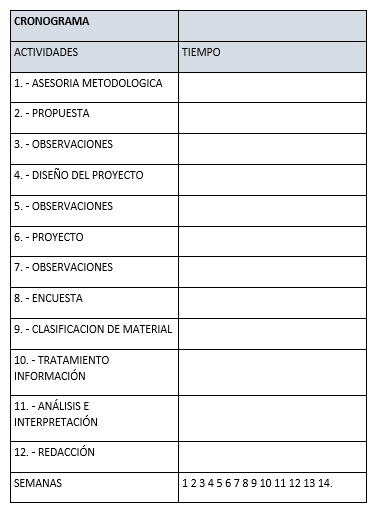
\includegraphics[scale=1]{imag11.PNG} 
\end{center}
 

\end{document}